\documentclass[conference]{IEEEtran}

\makeatletter
\newcommand{\rmnum}[1]{\romannumeral #1}
\newcommand{\Rmnum}[1]{\expandafter\@slowromancap\romannumeral #1@}
\makeatother

\usepackage{cite}
\usepackage{amsmath}
\usepackage{amsthm}

\newtheorem{theorem}{Theorem}
\newtheorem{lemma}[theorem]{Lemma}

\ifCLASSINFOpdf
   \usepackage[pdftex]{graphicx}
  % declare the path(s) where your graphic files are
   \graphicspath{{./png/}}
  % and their extensions so you won't have to specify these with
  % every instance of \includegraphics
   \DeclareGraphicsExtensions{.pdf,.png}
\else
  % or other class option (dvipsone, dvipdf, if not using dvips). graphicx
  % will default to the driver specified in the system graphics.cfg if no
  % driver is specified.
  % \usepackage[dvips]{graphicx}
  % declare the path(s) where your graphic files are
  % \graphicspath{{../eps/}}
  % and their extensions so you won't have to specify these with
  % every instance of \includegraphics
  % \DeclareGraphicsExtensions{.eps}
\fi

\ifCLASSOPTIONcompsoc
    \usepackage[caption=false,font=normalsize,labelfont=sf,textfont=sf]{subfig}
\else
    \usepackage[caption=false,font=footnotesize]{subfig}
\fi



% correct bad hyphenation here
\hyphenation{op-tical net-works semi-conduc-tor}
\newcommand{\ignore}[1]{{}}

\begin{document}

\title{Robust Energy-Aware Routing with Uncertain Traffic Demands}


\author{\IEEEauthorblockN{Heng Lin}
\IEEEauthorblockA{Tsinghua University \\ henglin1991@gmail.com}
\and
\IEEEauthorblockN{Mingwei Xu}
\IEEEauthorblockA{Tsinghua University \\ xmw@cernet.edu.cn}
\and
\IEEEauthorblockN{Yuan Yang}
\IEEEauthorblockA{Tsinghua University \\ yyang@csnet1.cs.tsinghua.edu.cn}}


% make the title area
\maketitle

% As a general rule, do not put math, special symbols or citations
% in the abstract
\begin{abstract}
Energy conservation has become a major challenge to the Internet. In existing approaches, a part of line cards
are switched into sleep mode for energy conservation, and the routing is configured carefully to balance energy saving
and traffic engineering goals, such as the maximum link utilization ratio (MLUR). Typically, traffic demands are
used as inputs, and routing is computed accordingly. However, accurate traffic matrices are difficult to obtain and
are changing frequently. This makes the approaches difficult to implement. Further, the routing may shift
frequently, and is not robust to sudden traffic changes.

In this paper, we propose a different approach that finds one energy-aware routing robust to a set of traffic
matrices, particularly to arbitrary traffic demands. Such a routing without energy consideration is known as
the demand-oblivious routing, and is well studied. However, the problem becomes much more challenging when energy
conservation is involved. To overcome the challenges, we first define a new metric, namely oblivious performance
ratio (OPR) with energy constraint, which reflects the MLUR distance from a routing to the optimal routing when
certain energy conservation requirement is satisfied. We model the problem of minimizing the performance ratio,
and analyze the lower and the upper bounds. Then, we propose Robust Energy-Aware Routing (REAR) to solve
the problem in two phases. REAR select sleeping links based on extended robust link utilization (ERLU) or algebraic
connectivity, and compute the routing based on a classical demand-oblivious routing algorithm.
We evaluate our algorithms on real and synthetic topologies. The simulation results show that REAR can save
19\% of line card power while the performance ratio is less than 34\%.
\end{abstract}

\IEEEpeerreviewmaketitle

\section{Introduction}

Energy conservation has become a global concern nowadays. The Internet is one of the major energy consumers, and its rapid growth makes the green Internet a hot research topic. In the Internet backbone, energy is mainly drawn by routers and switches. Such devices consume almost full power even if the traffic load is small. Thus, an effective method to save energy in the Internet is to aggregate traffic into part of the routers when the traffic load is small, and switch the under-utilized components (routers or line cards) into off/sleep mode. Such a method is known as the energy efficient routing.

An important issue for energy efficient routing is to avoid network congestion after the traffic is aggregated. Many approaches have been proposed in existing works. Most approaches compute the routing based on real-time traffic matrices or link loads, to achieve a good load balancing and avoid congestion. However, such approaches come at a cost of obtaining real-time traffic data. Furthermore, the routing may shift frequently with the traffic changes, and a sudden traffic change may still induce congestions. To this end, we need to study the robustness of energy efficient routing.

Specifically, we study the energy efficient routing when traffic matrices cannot be obtained or predicted precisely, i.e., with uncertain traffic demands. To achieve robustness, we need to find a routing, which can perform near optimally under a range of traffic matrices. The key technique that makes this possible is the advanced \emph{demand-oblivious routing}. A seminal work \cite{networking:oblivious} find that, the distance between the maximum link utilization ratio (MLUR) of a demand-oblivious routing and the MLUR of the optimal routing is bounded. Thus, no matter how the traffic demand changes, the demand-oblivious routing can guarantee certain performance. We note that this conclusion is in a network without off/sleep components, and we need to consider the situation when energy conservation is required.

However, existing demand-oblivious routing algorithms cannot be directly applied to energy efficient routing. There are several challenges. First, we need to define a metric that can effectively measure the distance between a robust energy efficient routing and the optimal routing, because the existing metric for demand-oblivious routing fails in the situation when some components are switched into off/sleep mode. Second, we need to analyze whether the metric can be bounded, just like for demand-oblivious routing. If there exists no bound, then it is not feasible to find a robust energy efficient routing. Third, we need practical algorithms to compute the robust energy efficient routing. Specifically, we need to determine: 1) which routers or line cards should be switched into off/sleep mode, to achieve energy efficiency; and 2) in which path to forward the traffic for robustness, while the path does not traverse the off/sleep components.

In this paper, we overcome the aforementioned challenges. First, we define a new metric, namely the oblivious performance ratio with energy constraint (OPRE). The OPRE reflects the MLUR distance from a routing to the optimal one when certain energy conservation requirement is satisfied. We model the problem of minimizing the OPRE. Second, we prove that there exists a robust energy efficient routing with the minimum OPRE, which has an upper bound given a network. Then, we propose Robust Energy-Aware Routing (REAR) scheme, which uses heuristic algorithms to solve the problem. We develop algorithm XXX, which chooses off/sleep line cards in a way that the OPRE can be minimized potentially. We then develop algorithm XXX to compute the routing in the remaining topology, by extending existing optimal demand-oblivious routing algorithm. We evaluate our algorithms by simulations on real topologies and synthetic traffic demands with random fluctuations. The results show that REAR can achieve an OPRE of 1.34 while 19\% of line card power is saved.

The rest of the paper is organized as follows. Section \Rmnum{2} shows the related work. Section \Rmnum{3} presents metric OPRE and formally models the problem. We presents the bounds on OPRE in Section \Rmnum{4}, and propose our algorithms in Section \Rmnum{5}. Section \Rmnum{6} shows our simulation setup and results, and Section \Rmnum{7} concludes our work.

\ignore{
Usually, We compute routing to stipulate how is the traffic going, to achieve some traffic engineering goals such as
the maximum link utilization ratio (MLUR). In details, we use traffic demands and network topology as input for
computation, then combine routing and traffic demands to get the traffic on each link, based on which we determind
which link can be put to sleep. However, measuring and predicting accurate traffic demands are difficult, so does its dynamic
natrue. Although we have obtained all knowledge about traffic demands, the corresponding routing may shift frequently
when the traffic demands change. It means that we should change the link (line cards) working mode frequently as well,
of course it is unpractical. So we need the routing be robust to sudden traffic changes, and based on the approximate traffic demands.
Such a routing is known as the demand-oblivious routing and is well studied in \cite{networking:oblivious}, which proposes
the algorithm for computing robust routing with uncertain traffic demands on specific topology.


Unfortunately, there is no metric in such robust routing to measure the importance of links, in another word, we have no
idea to put which link to sleep mode. Furthermore, when some links are switched off and the topology changed actually, but we
still have no idea for how to adjust the routing in result topology. Another challenge is that, to achieve the power saving
goals we may should switch off not only one link, and it is a classical NP-Hard problem. To overcome the challenges,
we define a metric namely extended robust link utilization (ERLU) to measure the traffic engineering natrue of link without real traffic
demands, and define oblivious performance ratio (OPR) to reflect the MLUR distance from a routing to the optimal one
when certain energy conservation requirement is satisfied. In our algorithm, we use algebraic connectivity \cite{networking:algebraic} and
ERLU as criterion to switch off links, and use OPR to adjust routing.


Our main contribution in this paper is three-fold. Firstly, we model the problem of minimizing the OPR, then
analyze the lower and the upper bounds. Secondly, we propose an heuristic algorithm named Robust Energy-Aware Routing (REAR)
to solve the problem in two phases, includes choosing links to sleep and adjusting routing. Thirdly, we implement our
algorithm on real topology and arbitrary traffic demands to observe the relationship between energy conservation and OPR. The
simulation results show that REAR can save 19\% power of line cards while OPR is less than 34\% in some topology. Also
we investigate the path stretching problem.


The rest of the paper is organized as follows. Section \Rmnum{2} reviews the related work and Section \Rmnum{3}
defines two metric and models our problem. Following we propose our algorithm in Section \Rmnum{4}. For clearer understanding
on our problem, we give two simple samples and prove the bounds in Section \Rmnum{5}. Experiments are discribed
and result are showed in Section \Rmnum{6}. We discuss issues and future work in Section \Rmnum{7}, then conclude our wok in
Section \Rmnum{8}}

\section{Related Work}
related work

\section{Problem Statement}

\subsection{Background of Demand-Oblivious Routing}

As mentioned above, demand-oblivious routing aims at finding one routing that performs near optimally under a range of traffic demands. In traffic engineering, a typical metric to evaluate routing performance is the maximum link utilization ratio (MLUR). Clearly, the MLUR is corresponded with a specified traffic matrix (TM). Demand-oblivious routing defines oblivious performance ratio (OPR) to evaluate the routing performance without the knowledge of TM. We briefly present the background.

Given a TM, the distance between a routing to the optimal one is defined as the ratio between their MLURs. Formally, a network is modeled as undirected graph $G(V, E)$, where $V$ is the set of vertices (nodes), and $E$ is the set of edges (links). Let $cap_{ij}$ denote the capacity of the link $(i, j) \in E$. Let $d_{ab}$ denote the traffic demand from origin node $a$ and destination node $b$, and $m$ denote the TM that contains $d_{ab}$ for all $a, b \in V$. Let $f^r_{ab}(i,j)$ be the fraction of $d_{ab}$ that is routed on link $(i, j)$ $(0 \leq f^r_{ab}(i,j) \leq 1)$, using routing $r$. Routing $r$ is specified by $f^r_{ab}(i,j)$ for all $a, b \in V$ and $(i, j) \in E$, and we will formally define routing consistency later in Section III.C. Let $U_{r, m, G}$ be the MLUR of routing $r$ under TM $m$. We have
\begin{equation}
	U_{r, m, G} = \max_{(i,j)\in E} \frac{\sum_{a,b} d_{ab}f^r_{ab}(i,j)}{cap_{ij}}.
\end{equation}
Let $P(\{ r \},\{ m \}, G)$ be the \emph{performance ratio} of routing $r$ under TM $m$, which reflects how far from the routing to the optimal one, and is defined as
\begin{equation}
	P(r,\{ m \}, G) = \frac{U_{r,m,G}}{\min_{r'} U_{r', m, G}}.
\end{equation}

The \emph{oblivious performance ratio} (OPR) for routing $r$ is defined by extending TM $m$ to a set of TMs $M$, where $M$ can be the set of all TMs. We have
\begin{equation}
	P(r, M, G) = \max_{m\in M} P(r, \{ m \}, G).
\end{equation}
The target of demand-oblivious routing is to find routing $r$ that minimizes OPR $P(\{ r \}, M, G)$. Such a ``robust'' routing is independent of a specific TM, but can perform near optimally. A seminal work \cite{networking:oblivious} uses linear programming to find the routing that minimizes the OPR, and finds that the optimal solution exists, which means that the OPR is bounded.

\subsection{Oblivious Performance Ratio with Energy Constraint}

With energy constraint, a network may have to switch part of line cards into off/sleep mode to save the total energy consumption. This changes the network topology and makes metric OPR fail to evaluate the robustness of a routing. We use an example to show this. Assume that $G$ is a cycle with $n$ unit capacity links. Then, the minimal OPR of $G$ is $2-2/n$ \cite{networking:oblivious}. Now we pruning one link from $G$ to save energy, and the topology changes to $G^*$. Because there is only one routing feasible in $G^*$, OPR $P(\{ r \}, M, G^*)$ equals 1. Since 1 is less than $2-2/n$ for $n > 2$, it means that the routing after pruning one link is more robust than before. However, it is false because there are less links and the network is more likely to be congested.

The intrinsic reason for such a ``fake robust'' is that the topology is not changing when performance ratio is computed in Eq. (2). To address this issue, we extend the definition of OPR. Formally, let $G^*$ be a sub-graph of $G$ that satisfies the energy constraint (We will formally define the energy constraint in Section III.C, i.e., Eq. (8)). Note that in this case, a path cannot traverse a off/sleeping link, so routing $r$ is limited by $G^*$ (Eq. (7) in Section III.C). The extended performance ratio is defined as
\begin{equation}
	P(r, \{ m \}, G, G^*) = \frac{U_{r,m,G^*}}{\min_{r'} U_{r', m, G}}.
\end{equation}
Let $P^*(r, M, G, G^*)$ be the \emph{oblivious performance ratio with energy constraint} (OPRE) for routing $r$. We define $P^*(r, M, G, G^*)$ by extending $m$ to $M$. Similar to Eq. (3), we have
\begin{equation}
	P^*(r, M, G, G^*) = \max_{m\in M} P(r, \{ m \}, G, G^*).
\end{equation}
Note that $G^*$ is used to achieve certain energy conservation target. For an energy conservation target, there may exist a set of different $G^*$, which result in different OPRE. We will show an example below. When there is no energy constraint, $G^*$ equals $G$, and Eq. (5) naturally reduces to Eq. (3).

\subsection{Example}

We show an example of our new metric OPRE. The network is shown in Fig. 1, where two nodes $a, b$ are connected by two links $l_1$ and $l_2$.{\footnote{When there are parallel links, we can add a virtual node in each parallel link to keep $G(V,E)$ as a simple graph.}} The capacities of the links are 3 Mbps and 4 Mbps, respectively. To forward a traffic demand of $d_{ab}$, the optimal routing is to put $\frac{3}{7}d_{ab}$ on link $l_1$ and $\frac{4}{7}d_{ab}$ on link $l_2$, which results in the MLUR of $\frac{1}{7}d_{ab}$. This routing is also the optimal demand-oblivious routing, because the routing is optimal no matter how $d_{ab}$ changes. Thus, the OPR equals 1.

\begin{figure}[!t]
\centering
\vspace*{0.1in}
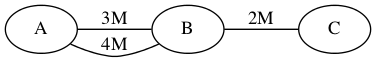
\includegraphics[width=6cm]{3-nodes-example}
\caption{Model Example. There is traffic demand $d_{ab}$ from $a$ to $b$.}
\label{label}
\vspace*{0.1in}
\end{figure}

Now, assume that links $l_1$ and $l_2$ consume the same power, and one link has to be switched off/sleep to save energy. Let us check the OPRE after pruning $l_1$ and $l_2$, respectively. If $l_1$ is pruned, $d_{ab}$ is put on link $l_2$, and the MLUR is $\frac{1}{4}d_{ab}$, so the OPRE is $\frac{1}{4}d_{ab}/\frac{1}{7}d_{ab} = 7/4 = 1.75$. If $l_2$ is pruned, $d_{ab}$ traverses link $l_1$, resulting in the MLUR of $\frac{1}{3}d_{ab}$, so the OPRE is $\frac{1}{3}d_{ab}/\frac{1}{7}d_{ab} = 7/3 = 2.33$. The results tell us that pruning link $l_1$ is more robust than pruning link $l_2$. This is consistent with the intuition that link $l_2$ has a larger capacity and is stronger against congestion.

\subsection{Problem Formulation}

Now we formally model the problem. Our objective is to minimize OPRE $P^*(r, M, G, G^*)$, where $M$ and $G$ are inputs, and routing $r$ and sub-graph $G^*$ are decision variables. The Min-OPRE problem is as follows.

\begin{center}
Minimize \quad $P^*(r, M, G, G^*)$
\end{center}

\begin{center}
s.t. (1),\ (4),\ (5)
\end{center}

\begin{center}
    $\forall a,b,i \in V$: \quad \quad \quad \quad \quad \quad \quad \quad \quad \quad \quad \quad \quad \quad \quad
    \vspace{-0.3in}
\end{center}

\begin{equation}
    \begin{split}
    \sum_{j, s.t.(i,j) \in E}\hspace{-0.2in}f^{r'}_{ab}(i,j) - \hspace{-0.2in}\sum_{j, s.t.(j,i) \in E}\hspace{-0.2in}f^{r'}_{ab}(j,i) =
    \left\{
        \begin{array}{c}
        \ \ 1, \ i = a \\
        -1, \ i = b \\
        \ \ \ \ \ 0, \ i \neq a,b \\
        \end{array}
    \right.
    \end{split}
\end{equation}

\begin{center}
    \vspace{0.1in}
    $\forall a,b,i \in V$: \quad \quad \quad \quad \quad \quad \quad \quad \quad \quad \quad \quad \quad \quad \quad
    \vspace{-0.3in}
\end{center}

\begin{equation}
    \begin{split}
    \sum_{j, s.t.(i,j) \in E^*}\hspace{-0.2in}f^r_{ab}(i,j) - \hspace{-0.3in}\sum_{j, s.t.(j,i) \in E^*}\hspace{-0.2in}f^r_{ab}(j,i) =
    \left\{
        \begin{array}{c}
        \ \ 1, \ i = a \\
        -1, \ i = b \\
        \ \ \ \ \ 0, \ i \neq a,b \\
        \end{array}
    \right.
    \end{split}
\end{equation}

\begin{center}
    \vspace{0.1in}
    $\forall a,b \in V$, $\forall i,j \in E$: \quad \quad \quad \quad \quad \quad \quad \quad \quad \quad \quad 
    \vspace{-0.15in}
\end{center}

\begin{equation}
    0 \leq f^r_{ab}(i,j),f^{r'}_{ab}(i,j) \leq 1
\end{equation}

\begin{equation}
    \sum_{l \in E^*} p(l) / \sum_{l \in E} p(l) \leq 1 - \theta
\end{equation}

Constraints (1), (4), and (5) follow our definition of the OPRE. Eq. (6) means that the optimal routing $r'$ in $G$ must be a valid routing, i.e. with routing consistency. Specifically, for the source/destination node, all traffic must be routed/received; and for an intermediate node, the traffic flowing out must equal the traffic flowing in. Similarly, Eq. (7) means that the robust routing $r$ in $G^*$ must be a valid routing. Ineq. (8) means that the range of $f^r_{ab}(i,j)$ and $f^{r'}_{ab}(i,j)$ is from 0 to 1. Ineq. (9) means that the power consumption of links in $G^*$ must be less than a given threshold. In Ineq. (9), $\theta$ denotes the power saving ratio we must achieve by using $G^*$. Here, we use $p(l)$ to denote the power consumption of link $l$, which is mainly drawn by the line cards at the two ends of the link. Note that $p(l)$ is independent of the traffic volume, and this assumption is based on the fact that in current stage, the power of a line card changes little with the traffic volume \cite{networking:hopbyhop}.

Note that if $G^* = G$ satisfy the energy constraint Ineq. (9) and $M$ is the set of all TMs, the Min-OPRE problem reduces to the demand-oblivious routing problem, and can be transformed into a linear program and solved in polynomial time \cite{networking:oblivious}. However, we must find the optimal $G^*$ to achieve the required power saving ratio in other cases, and Min-OPRE is an MILP and is NP-hard in general.

Also note that we put the power saving in the constraint of our problem, instead of the objective function. In such a way, we can balance the trade off between energy conservation and the OPRE, by setting different values of power saving ratio $\theta$. We can even achieve the maximum power saving ratio by a binary search on $\theta$.

\section{Upper Bounds of the Minimum OPRE}

In this section, we analyze the upper bounds of the minimum OPRE. We are interested in two extreme types of networks, i.e., cycles and cliques, because general networks can be seen as intermediate cases between them. We will present the upper bounds with small and large values of $\theta$. We find that, though the minimum OPR of cycles and cliques is similar and bounded by 2 \cite{networking:oblivious}, the minimum OPRE is much more different and has a larger upper bound with a larger $\theta$. These theoretical results tell us that the robust energy efficient routing exists, and tell us how close a robust routing can get to the optimal routing.

\begin{lemma}
$\min P^*(r, M, G, G^*) \geq \min P^*(r, M, G)$ if $G^* \subseteq G$, where the equation holds if $G^* = G$.
\end{lemma}
\begin{proof}
We assume exist a $G^*$, s.t. min $P^*(r,M,G,G^*)$ $<$ min $P^*(r, M, G)$. Becuase $G^*$ is the subset of $G$, we directly
use the robust routing of $G^*$ to $G$, then $P^*(r, M, G)$ will equal to $P^*(r,M,G,G^*)$, and arise contradiction.
Particularly, when $G^* = G$, $G^*$ is the subset of $G$, and $G$ is the subset of $G^*$, so there is both 
min $P^*(r,M,G,G^*)$ $\geq$ min $P^*(r, M, G)$ and $P^*(r, M ,G)$ $\geq$ $P^*(r, M, G, G^*)$, so they are equal to each other 
when $G^*$ = $G$. This ends our proof.
\end{proof}

\begin{theorem}
The minimum OPRE of $C_n$ (the cycle on $n$ vertices with unit capacity links) and $K_n$ (the complete graph on $n$ vertices with unit capacity links) is $2-2/n$ if $\theta = 0$.
\end{theorem}
\begin{proof}
According to Lemma 1, the minimum OPRE of $C_n$ is the minimum OPR, i.e., $\min P^*(r, M, C_n)$, when $\theta = 0$. Similarly, the minimum OPRE of $K_n$ is $\min P^*(r, M, K_n)$ when $\theta = 0$. On the other hand, we know from \cite{networking:oblivious} that the minimum OPR of $C_n$ is $2-2/n$, and the minimum OPR of $K_n$ is also $2-2/n$. This ends our proof.
\end{proof}

Theorem 2 shows the minimum OPRE when $\theta = 0$ and all link capacities are the same. In a more general case when there are different link capacities, we have

\begin{theorem}
The upper bound of the minimum OPRE for a cycle on $n$ nodes is $1 + \frac{\max cap_{ij}}{\min cap_{ij}}$ if $\theta = 0$.
\end{theorem}
\begin{proof}
See Appendix A.
\end{proof}

\begin{theorem}
The upper bound of the minimum OPRE for a complete graph on $n$ nodes is $1 + \frac{\max cap_{ij}}{\min cap_{ij}}$ if $\theta = 0$.
\end{theorem}
\begin{proof}
See Appendix A.
\end{proof}

Theorem 3 and Theorem 4 tell us that the minimum OPRE is related to the link capacity difference in the network. The above results are for $\theta = 0$. Now let us see the results for a large $\theta$. Since there is not much difference between the power consumptions for links with different capacities \cite{}, we consider the spanning trees of a graph, which can achieve a near-optimal $\theta$. We have
\begin{theorem}
Let $G^*$ be a spanning tree of a cycle on $n$ nodes, and then the upper bound of the OPRE is $1 + \frac{\max cap_{ij}}{\min cap_{ij}}$.
\end{theorem}
\begin{proof}
See Appendix B.
\end{proof}
\begin{theorem}
Let $G^*$ be a spanning tree of a complete graph on $n$ nodes, and then the upper bound of the OPRE is $\frac{n^2}{2} \frac{\max cap_{ij}}{\min cap_{ij}}$.
\end{theorem}
\begin{proof}
See Appendix C.
\end{proof}

Theorem 5 and Theorem 6 present a large gap between the OPRE upper bounds in the two types of networks, because when $G^*$ is a spanning tree, more links are pruned in the complete graph. This implies that in order to achieve more energy conservation, the OPRE may become larger quickly, and the routing becomes less robust, in the worst case. However, we can still develop effective algorithms to achieve a small OPRE and save energy in general cases, i.e., in real-world networks which have much less link densities than a complete graph.


\section{Robust Energy-Aware Routing Algorithms}

In our paper, Robust Energy-Aware Routing (REAR) algorithm works in two phases. Firstly, REAR select links
should be put to sleep from the origin topology based on extended robust link utilization (ERLU),
then compute the robust routing based on demand-oblivious routing algorithm.

\subsection{Extended Robust Link Utilization}
The demand-oblivious routing is not always the best one for specific $TM$, but good enough for a range of $TM$.
we mentioned the definition of link utilization above when demand and routing are determined, as demand become
oblivious, the definition is also not suitable. So we define a notation named extended robust link utilization (ERLU)
replace the normal link utilization like :

\begin{equation}
	u^e_{ij} = \frac {\sum_{a,b}f_{ab}(i,j)} {cap_{ij}}
\end{equation}


Proposing this definition for two consideration: firstly, the more flows across the link, the greater the $u^e_{ij}$ is;
secondly, the more fraction of one flow across the link, the greater the $u^e_{ij}$ is. The link with greater
ERLU is also more important than others in a sense. Although there is no demand here, we mean
there is more probability that this link have greater link utilization when specific demand come.

\subsection{Algorithm Phase One}
REAR sleep as many links as possible without losing connectivity of graph.
Originly,  we should calculate ERLU of all the links and sleep the lowest one from the graph, then repeat calculate and remove
process until arrive some specific threhold. Obviously, it is NP-Hard, following is a heuristic algorithm.


For the origin graph, we calculate the ERLU of every link, and then sort these values
from small to big, output ordered list denoted as $\Gamma$:
\begin{equation}
	\Gamma = \{..., l_i, ..., l_j, ...\}
\end{equation}
where $u^e_{l_i} < u^e_{l_j}$.


Pay attention we only compute the ERLU once at the begining of algorihtm, and the ordered list $\Gamma$ show
the order of `importance' among links in the graph.


Now we begin selecting which link should be sleep.
We denote the set of the sleeping links as $S$, and the output of this phase is final graph $G^* = (V, E-S)$. We set
$S = \emptyset$, and repeat our selecting process, each iteration we select one link, remove it from $\Gamma$ and put it into $S$.
In iteration $i$, algorithm scan links as the order in $\Gamma$, we try to
remove this link from the graph to check if the graph is still connected and the energy conservation have not arrive the threshold.
If so, we select it then go next iteration.
Otherwise choose the next link from $\Gamma$ for trying to remove. Algorithm
stop until all the links in $\Gamma$ is tried but no one is satisfied with both connectivity and power threhold.


But before going ahead our algorithm, there is another thing we should care, how to measure the power of graph.
We simple take an power model from \cite{networking:greente} showed in Table \Rmnum{2}, and defined the difference of power consumption
between two graphs as:
\begin{equation}
	diff_p = 1 - \theta = \frac{\rho(G_{S, l}^o)} {\rho(G^o)} * 100
\end{equation}
where $\rho(G_{S, l}^o)$ is the power consumption of the final graph, when the links set $S$ and
link $l$ are both removed from the origin graph $G^o$, and the $\rho(G^o)$ is the power consumption of
the origin graph.


If we set $diff_p$ valued 90\%, it means that whenever we try to remove the link $l$ from the origin graph in
iteration, the power consumption should never lower than the 90\% of origin one. Following is our implementation:


\begin{table}[!th]
\begin{tabular}{ll}
\hline
\textbf{Algorithm REAR : Phase One}\\
\hline
$\:\:$\textbf{Input:} $G(V, E)$, $threhold$;\\
$\:\:$\textbf{Output:} $S$ in which links should be switched off;\\
$\quad\qquad\quad$ $G(V, E-S)$ which is the final network topology;\\
$\:\:$1:\ \textbf{for} {each link $l$ in $E$}\\
$\:\:$2:\quad\ $\Gamma[l] \leftarrow u^e_l$;\\
$\:\:$3:\ Resort $\Gamma$ in increasing order based on $u^e_l$;\\
$\:\:$4:\ $S \leftarrow \emptyset$, $goon \leftarrow true$;\\
$\:\:$5:\ \textbf{while} {$goon$}\\
$\:\:$6:\quad\  $goon \leftarrow false$;\\
$\:\:$7:\quad\ \textbf{for} {each link $l$ in $\Gamma - S$}\\
$\:\:$8:\quad\ \quad\ \textbf{if} $G_{S,l}$ is connected and $\rho(G_{S,l})/\rho(G)>threhold$\\
$\:\:$9:\quad\ \quad\ \quad\ $S \leftarrow S \cup \{l\}$;\\
$\:\:$10:\quad\ \quad\ \quad\ $goon \leftarrow true$;\\
$\:\:$11:\quad\ \quad\ \quad\ \textbf{break};\\
$\:\:$12:\ \textbf{return} $S, G(V, E-S)$;\\
\hline
\end{tabular}
\end{table}



\subsection{Algorihtm Phase Two}
Once we get the output network topology from the first phase, it is time to compute
the robust routing. On one hand, computation process may cost too much time if we directly calculate the robust routing in
the final graph; on the other hand, the robust routing based on the final graph may not be the best one.
There is a heuristic algorithm
based on the demand-oblivious routing on the origin graph, which should be obtained at first.
then adjust routing in details according to the links we switched off.


The demand-oblivious routing can be computed by a single LP with $O(mn^2)$ variables and $O(nm^2)$ constraints[1] :
\begin{table}[!th]
\begin{tabular}{ll}
$\:\:$\quad\quad\quad\quad\ \textbf{min} $r$ \\
$\:\:$\quad\quad\quad\quad\ $f_{ij}(e)$ is a routing \\
$\:\:$\quad\quad\quad\quad\ $\forall$ links $l$: $\sum_m cap(m)t(l,m) \le r$ \\
$\:\:$\quad\quad\quad\quad\ $\forall$ links $l$, $\forall$ pairs $i \rightarrow j$: \\
$\:\:$\quad\quad\quad\quad\quad\quad\ $f_{ij}(l)/cap(l) \le p_l(i,j)$ \\
$\:\:$\quad\quad\quad\quad\ $\forall$ links $l$, $\forall$ nodes $i$, $\forall$ edges $e = j \rightarrow k$: \\
$\:\:$\quad\quad\quad\quad\quad\quad\ $\pi(l, link-of(e)) + p_l(i,j) - p_l(i,k) \ge 0$ \\
$\:\:$\quad\quad\quad\quad\ $\forall$ links $l$, $m$: $\pi(l, m) \ge 0$ \\
$\:\:$\quad\quad\quad\quad\ $\forall$ links $l$, $\forall$ nodes $i$: $p_l(i,i) = 0$ \\
$\:\:$\quad\quad\quad\quad\ $\forall$ links $l$, $\forall$ nodes $i$, $j$: $p_l(i,j) \ge 0$ \\
\end{tabular}
\end{table}


where the $cap(l)$ is the capacity of link $l$;
and $\pi(l,m)$ is the weights for every pair of links $l$, $m$; and the variables $p_l(i,j)$ for each link $l$
and OD pair $i$, $j$ is the length of the shortest path from $i$ to $j$ according to the link weights $\pi(l, m)$.


The routing we get indicate how to arrive at destination node from source node for every OD pair in the origin topology.
What is different is that, the flow can be splited in the routing, i.e. there may be two paths ($path_1$, $path_2$)
both from source node $s$ to destination node $d$, and the optimal obilious routing trace 70\% traffic on
$path_1$ and left on $path_2$. Although splitting flow is hard handled, we take a transformation for the case like that:
when an flow is coming, there is 70\% probability we trace it on $path_1$, otherwise $path_2$. This is easily implementated
in real world.


Because all the routing is based on the origin topology, when some links are switched off, we must adjust the routing
as well. Supposed there are some paths between two vertices $s$ and $d$, maybe one link in some paths be removed,
and these paths become not reachable any more, we should adjust the traffic in these paths to other paths. Of course,
we can not put the whole traffic on another path, this will make some links of the path congested, so we should split the traffic
to some paths `averagely`, in the sense of extended robust link utilization. Similarly to link utilization, we define the extended
robust link utilization as the maximum extended robust link utilization of links.


Take pair $(s, d)$ for example, routing includes paths from $s$ to $d$, such as $p_1, p_2, ... , p_n$. While only $p_1$ trace
the removed link, and of course it will be unreachable. We split the traffic of $p_1$, and put them on other paths to make
the extend robust link utilization of paths almost closely.


And this is our implementation:
\begin{table}[!th]
\begin{tabular}{ll}
\hline
\textbf{Algorithm REAR : Phase Two}\\
\hline
$\:\:$\textbf{Input:} $G(V,E)$ which is the origin topology;\\
$\quad\quad\ \ \ $ $S$ which is the switch-off links set generated by Phase One;\\
$\quad\quad\ \ \ $ $R$ which is the Robust Routing on origin topology;\\
$\:\:$\textbf{Output:} $Routing$ Robust Energy-Aware Routing on new topology\\
$\:\:$\ 1:\ $G^* \leftarrow G(V, E-S)$;\\
$\:\:$\ 2:\ \textbf{for} {each link $l$ in $S$}\\
$\:\:$\ 3:\quad\ \textbf{for} {each $s,d,paths$ in $R$}\\
$\:\:$\ 4:\quad\ \quad\ $traffic \leftarrow$ 0;\\
$\:\:$\ 5:\quad\ \quad\ \textbf{for} {each $path$ in $paths$}\\
$\:\:$\ 6:\quad\ \quad\ \quad\ \textbf{if} {$link$ in $path$}\\
$\:\:$\ 7:\quad\ \quad\ \quad\ \quad\ $traffic \leftarrow$ $traffic$ + $path$.$traffic$; \\
$\:\:$\ 8:\quad\ \quad\ \quad\ \quad\ $paths$.remove($path$); \\
$\:\:$\ 9:\quad\ \quad\ $yen\_paths \leftarrow$ yens\_algorithm($G^*$, $s$,$d$);\\
$\:\:$10:\quad\ \quad\ \textbf{while} {$traffic$ != 0}\\
$\:\:$11:\quad\ \quad\ \quad\ sort\_paths\_by\_extend\_robust\_link\_utilization($yen\_paths$)\\
$\:\:$12:\quad\ \quad\ \quad\ $yen\_paths$[0].$traffic$ = $traffic$ / N\\
$\:\:$13:\quad\ \quad\ \quad\ $traffic$ = $traffic$ - $traffic$ / N\\
$\:\:$14:\quad\ \quad\ \quad\ $paths$.add($yen\_paths$[0])\\
$\:\:$15:\quad\ \quad\ $paths$.merge();\\
$\:\:$16:\ \textbf{return} $R$;\\
\hline
\end{tabular}
\end{table}



\begin{figure*}[!t]
\centering
\vspace*{0.1in}
\subfloat{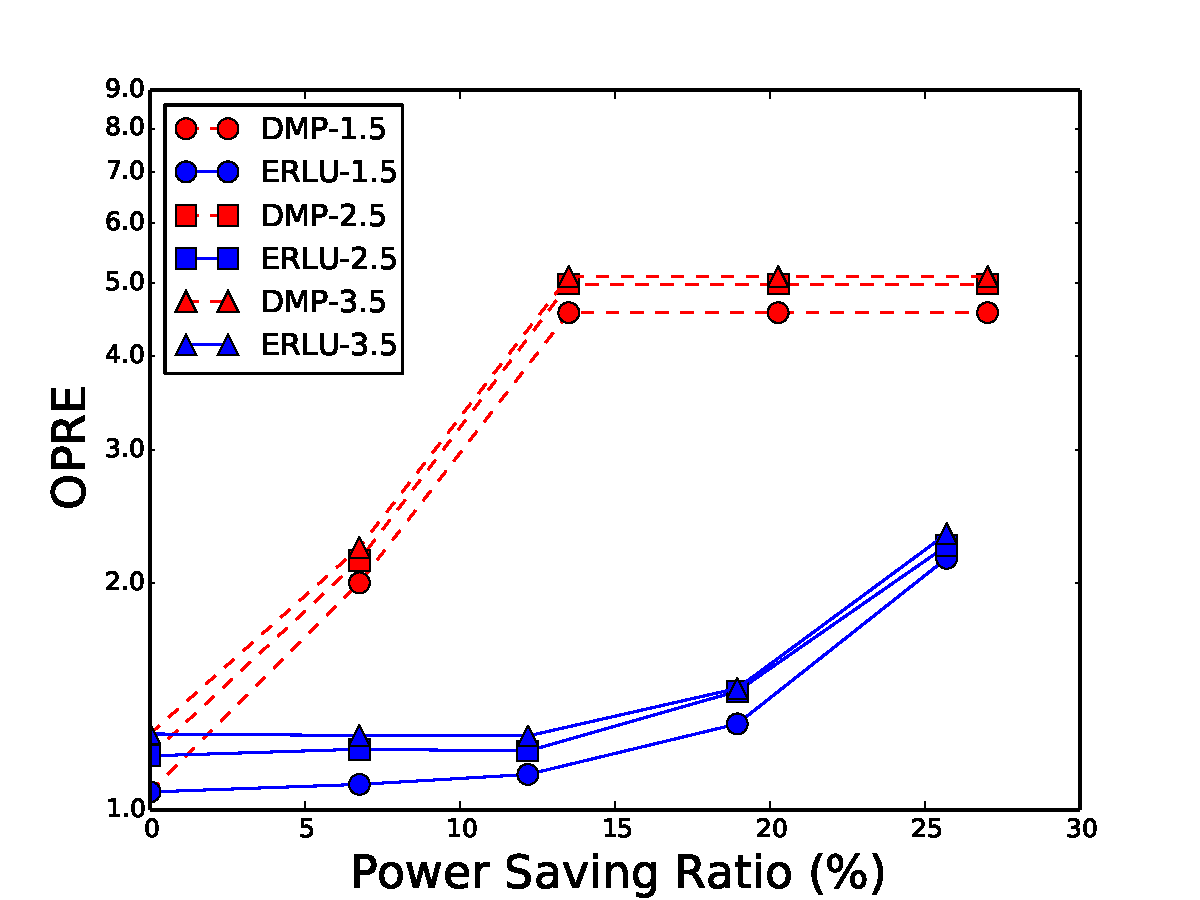
\includegraphics[width=6cm]{opr_with_power_abilene}}
\subfloat{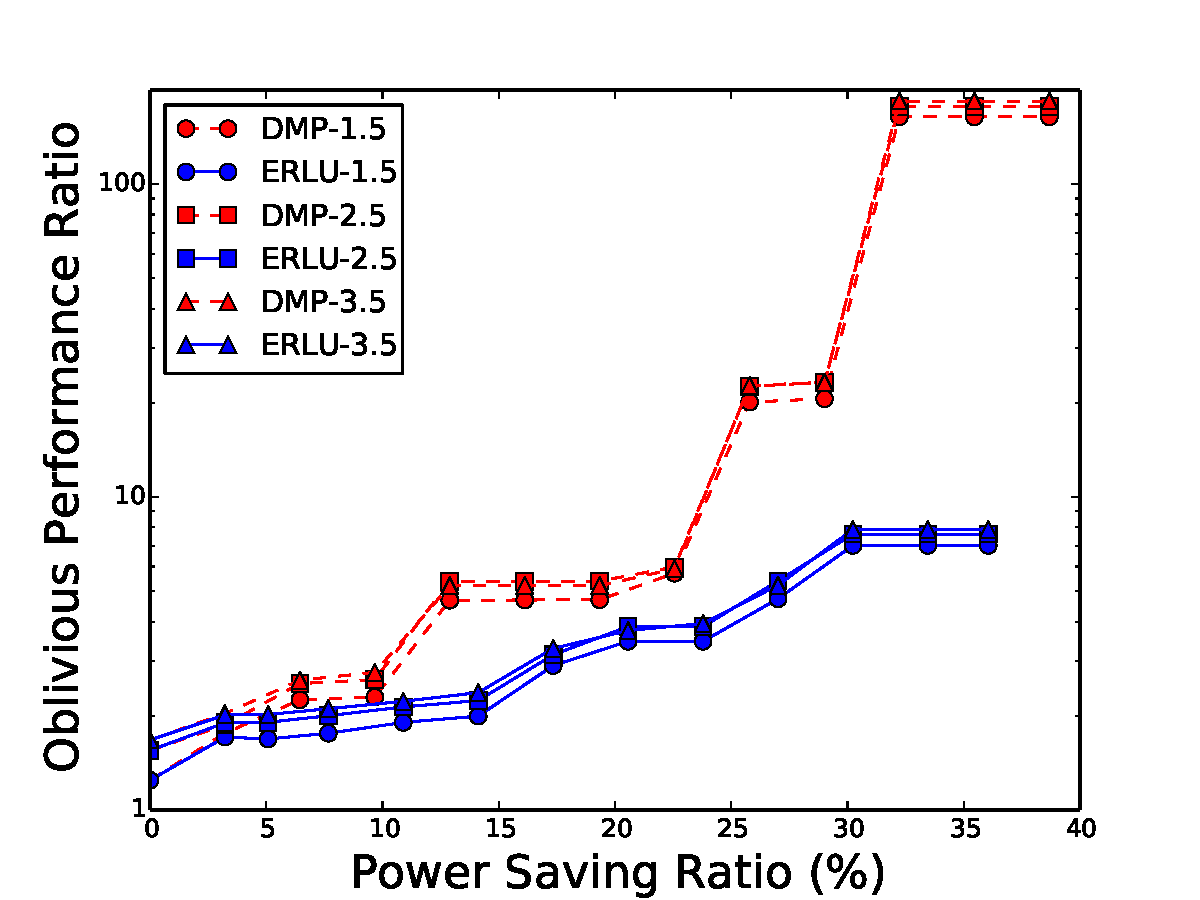
\includegraphics[width=6cm]{opr_with_power_geant}}
\subfloat{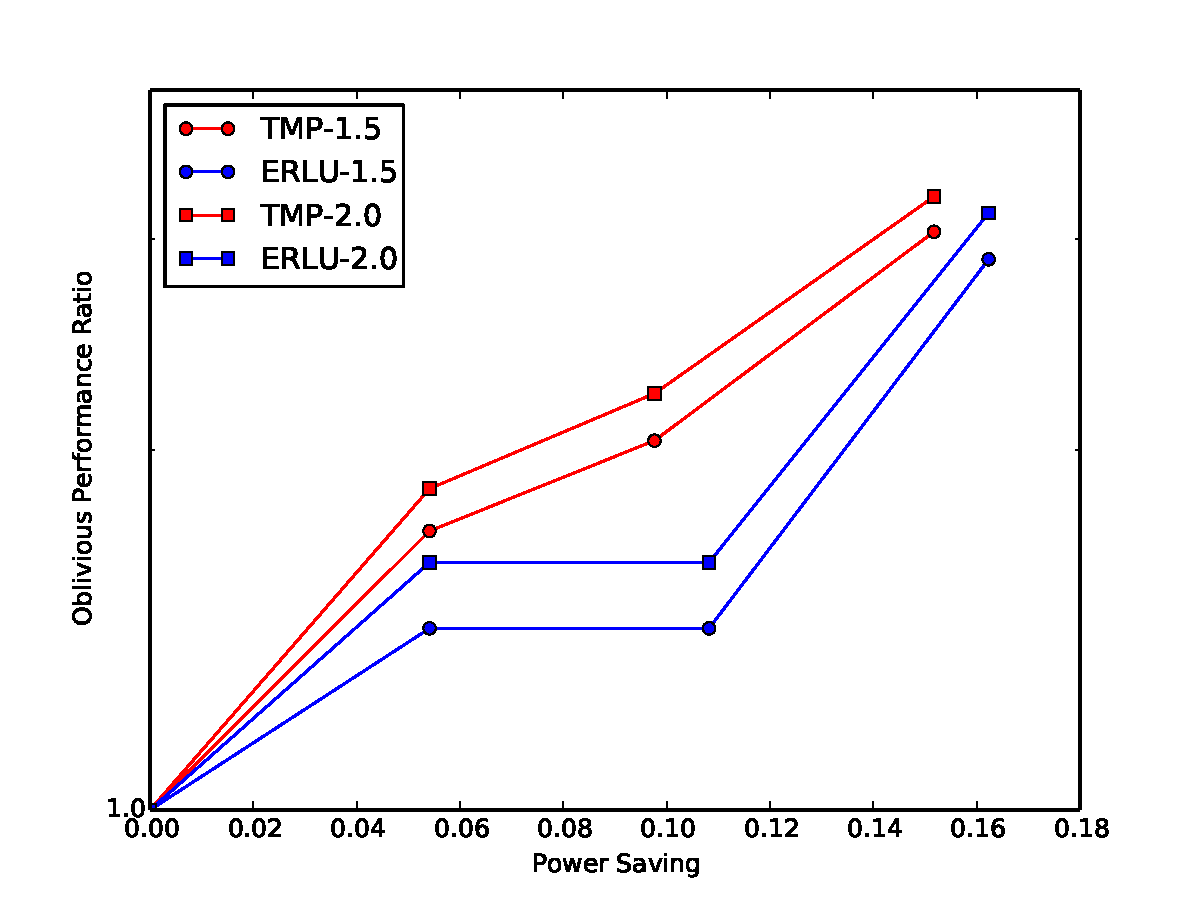
\includegraphics[width=6cm]{opr_with_power_cernet2}}
\caption{OPRE versus Power Saving: (1). Abilene, (b). Geant, (c). Cernet2}
\vspace*{0.1in}
\end{figure*}

\begin{figure*}[!t]
\centering
\vspace*{0.1in}
\subfloat{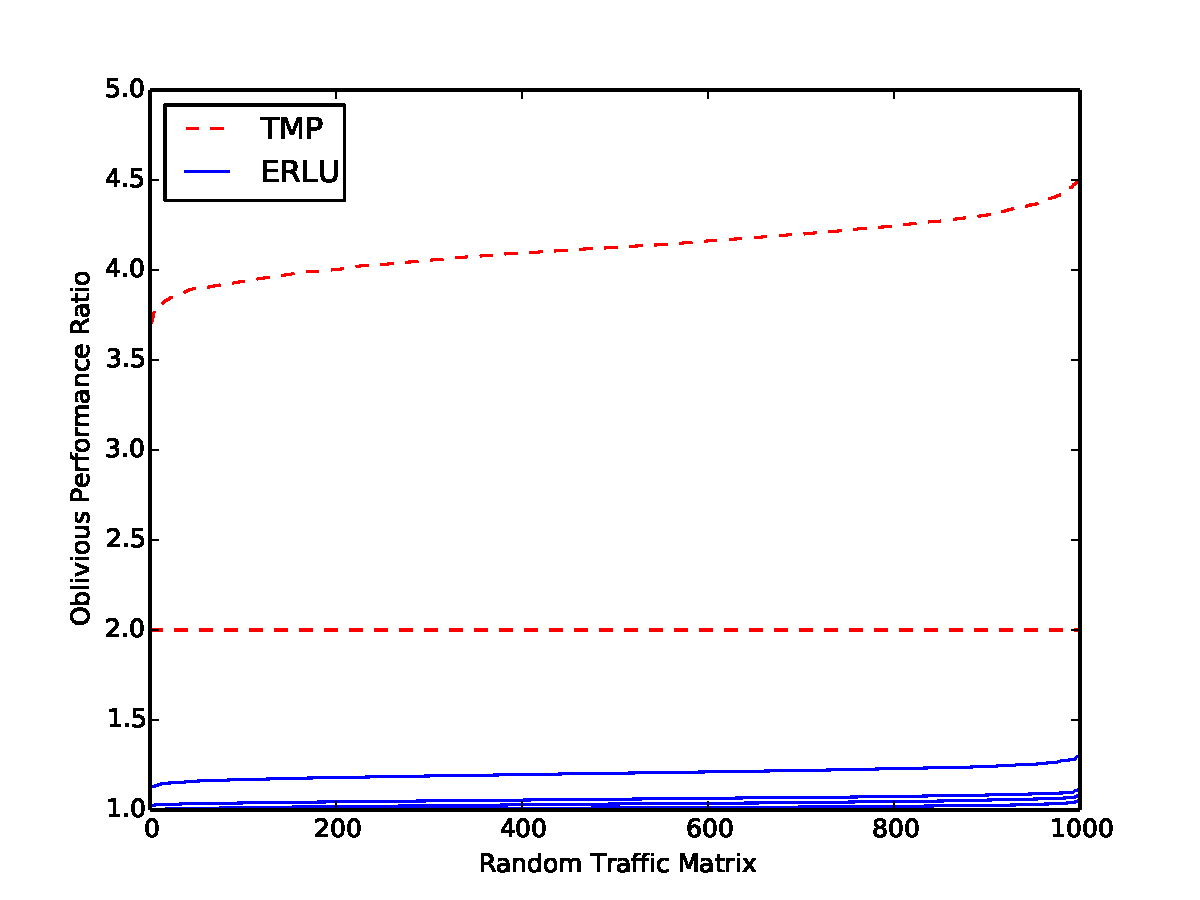
\includegraphics[width=6cm]{exp2_sort_abilene}}
\subfloat{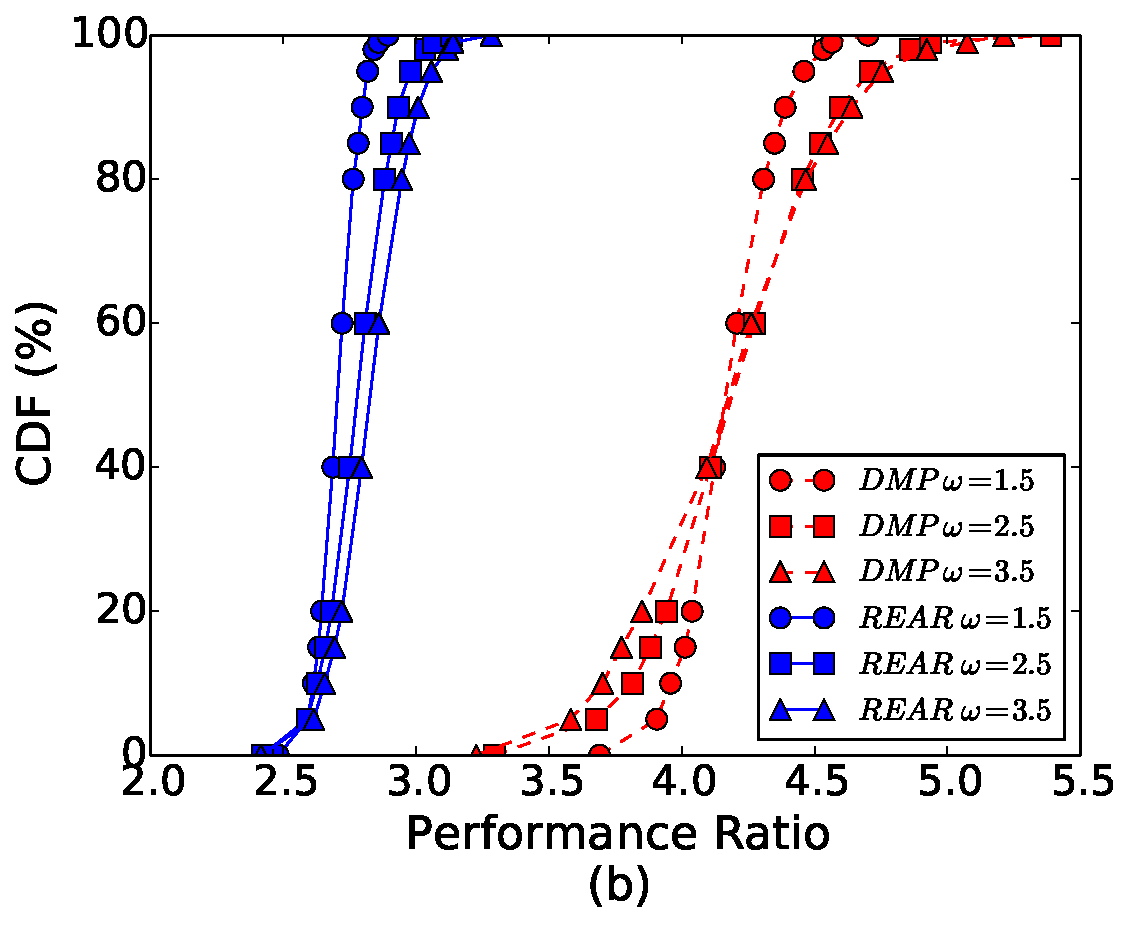
\includegraphics[width=6cm]{exp2_sort_geant}}
\subfloat{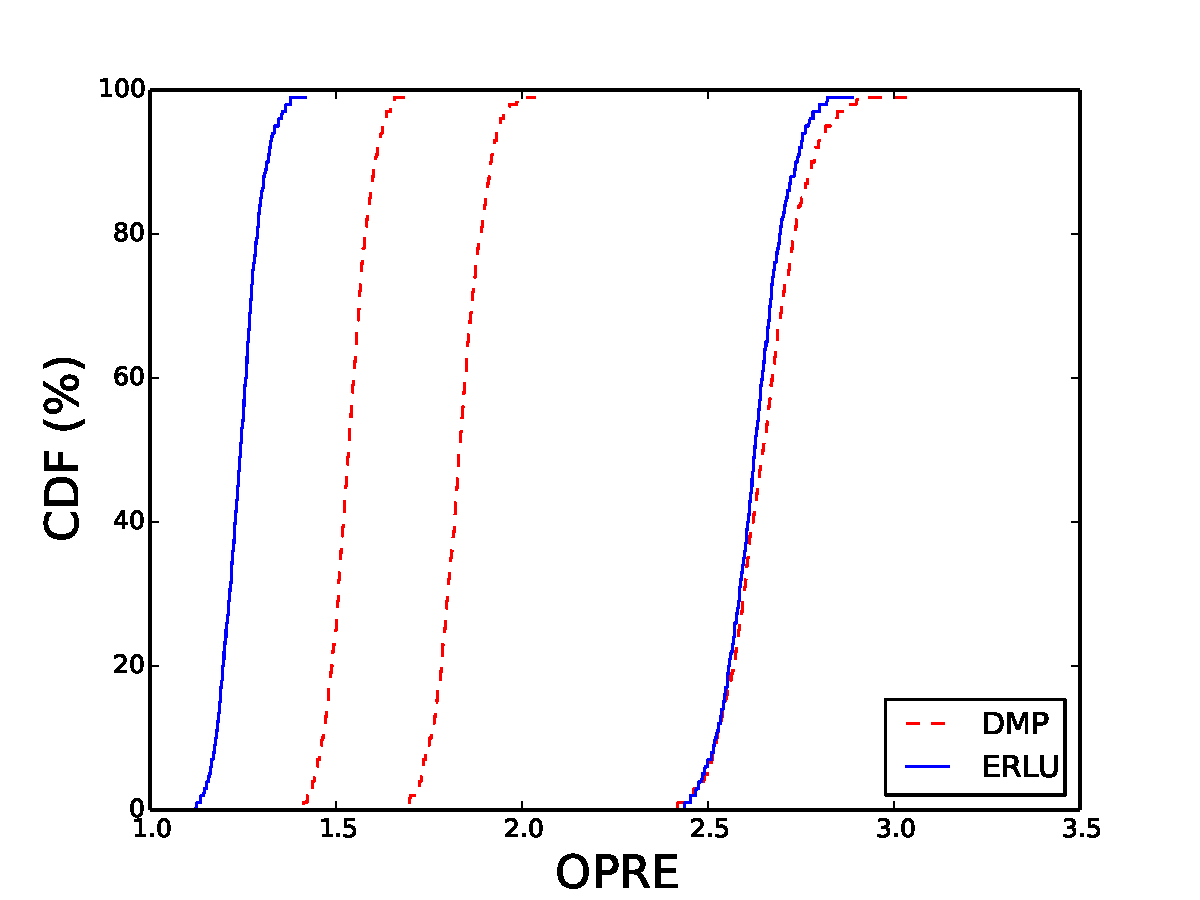
\includegraphics[width=6cm]{exp2_sort_cernet2}}
\caption{OPRE versus TMs: (a). Abilene, (b). Geant, (c). Cernet2}
\vspace*{0.1in}
\end{figure*}


\section{Experiments and Results}
We simulated our algorithm on real world topology, including Abilene, Geant and Cernet2, whose number of nodes and links are listed in Table \Rmnum{1}.
Then we generate random traffic matrix with Gravity Model \cite{networking:gravity}, which assume that the traffic demand between nodes is proportional
to their combined capacity of connecting links. To extrapolate a complete TM, we take an attribute margin $w$ to scale the traffic range from $1/w$ to $w$
base on the basic traffic demand. Particularly, when the $w$ limit extremity, we say the traffic matrix is really arbitrary, and our
algorithm is irrelevant with traffic.

\begin{table}[!t]
\renewcommand{\arraystretch}{1}
\caption{Topologies}
\label{three topologies}
\centering
\begin{tabular}{|c|c|c|c|}
\hline
\bfseries Topology & \bfseries Nodes & \bfseries Links & \bfseries Links can be Removed \\
\hline
Abilene & 12 & 15 & 4 \\
\hline
Geant & 23 & 37 & 15 \\
\hline
Cernet2 & 20 & 22 & 3 \\
\hline
\end{tabular}
\end{table}


\begin{figure*}[!t]
\centering
\vspace*{0.1in}
\subfloat{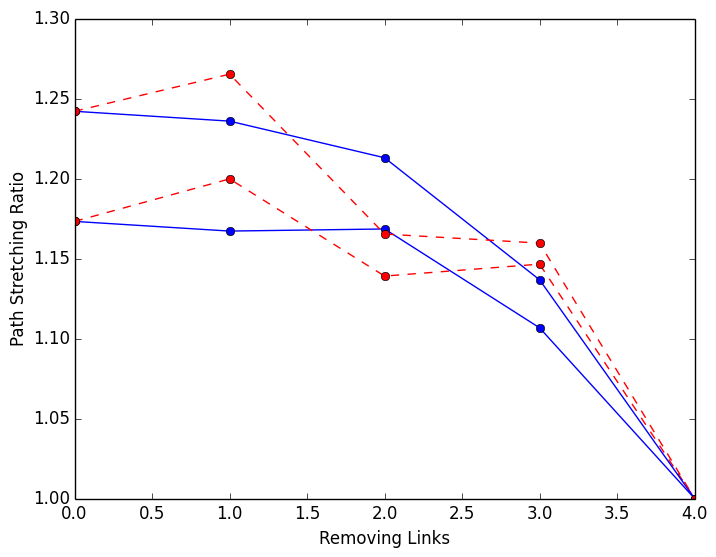
\includegraphics[width=6cm]{exp4_path_abilene}}
\subfloat{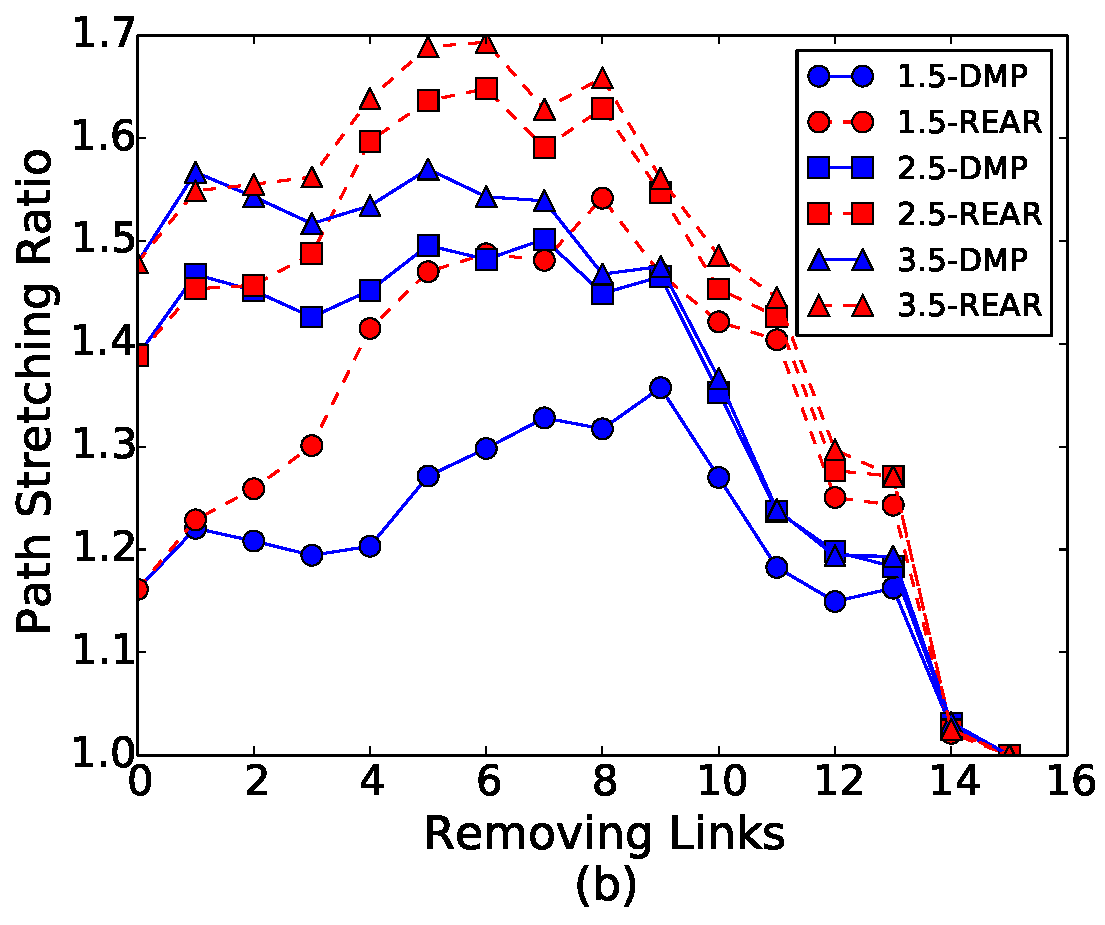
\includegraphics[width=6cm]{exp4_path_geant}}
\subfloat{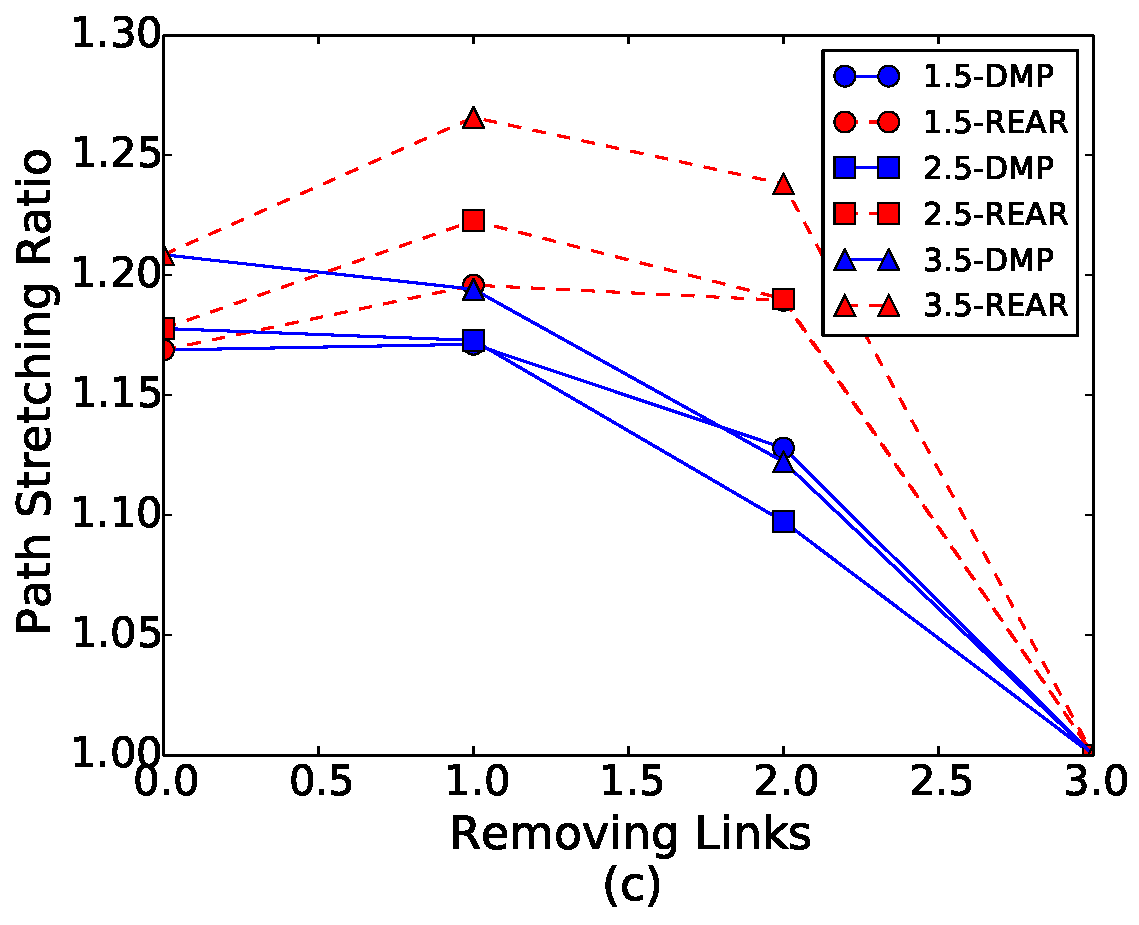
\includegraphics[width=6cm]{exp4_path_cernet2}}
\caption{Path Stretching: (a). Abilene, (b). Geant, (c). Cernet2}
\vspace*{0.1in}
\end{figure*}

\subsection{OPRE versus Power Saving}
In Figure 3, we see that the value of OPRE is at least 1 for all topologies even no links removed, particularly in Geant the value is 1.24,
it means the robust routing always not be the optimal for all TMs. It is reasonable because our robust routing is used for a range of traffic
rather than a specific TM.


When we switch off links, the topology lose connectivity and some routing paths will be failed, traffic on those paths will be
adjusted to others, which result in the value of OPRE increased. We take margin from 1.5 to 3.5 and observe this phenomena from Figure.
Pay attention that we scale the y-axis as logarithm for comparing DMP and ERLU in one figure. Intuitively, we can see ERLU is always
better than DMP whatever margin or power saving target is, because ERLU consider much more than DMP, such as capacity and robust traffic
flows. Another information from Figure 4 is that, we should carefully set the value of power saving for avoiding removing too much
links, which result in the OPRE increases rapidly, induce network congestions easily and make the robust routing be less `robust'.


we concern more about how is the OPRE varifying when achived specific power saving target. Obviously, the more links we removed,
the more power we saved, but how to quantify the power of one link is difficult. Green TE proposed a simple power model \cite{networking:greente},
which can be represented in Table \Rmnum{2}. In which, the total energy of topology is dominant by line cards of routers or switches,
when saying switch off the links we mean put down the according line cards.

\begin{table}[!t]
\renewcommand{\arraystretch}{1}
\caption{Green TE Power Model}
\label{power model}
\centering
\begin{tabular}{|c|c|c|}
\hline
\bfseries Line-Card & \bfseries Speed(Mbps) & \bfseries Power(Watts) \\
\hline
1-Port OC3 & 155.52 & 60 \\
\hline
8-Port OC3 & 1244.16 & 100 \\
\hline
1-Port OC48 & 2488.32 & 140 \\
\hline
1-Port OC192 & 9953.28 & 174 \\
\hline
\end{tabular}
\end{table}

We compute the power saving ratio as the total power of the removed links over the total power of all the links.
In Figure 3 (a), it shows we can save 19\% energy only with an OPRE of 1.30 in Abilene topology, and in Geant and Cernet2,
the OPRE is little higher. Curves present some scalariform, it means that in some range of power saving, the OPRE rise slowly,
and in the end of range, the energy conservation is efficient.


\subsection{OPRE versus Margin}
We take the margin $w$ as one of the input for computing robust routing, and margin identify a range of TMs the routing is
robust for. Once the $w$ limit extremely, our robust routing is said without knowledge of traffic matrix. Figure 3 shows the
OPRE increases little as $w$ increases, particularly in Geant, the difference almost can not be observed. It is obvious because
when the $w$ is greater, the traffic matrix is random in more wider range, and our OPRE may achieve worse case with more probability.


\subsection{OPRE versus TMs}
To simulate the worst case, we generate 1000 traffic matrices for every topoloy with margin attribute $w$. Figure 4 shows
the OPRE distribution in the process of experiment. For avoiding mess result from too many lines, we just show the first
three lines and the base line, which shows the distribution when no links is removed, i.e. seven lines in each figure.


In Figure 4 (a), we can only observe five lines because there are two overlapping lines, which means that when removing
links the worst case for the robust routing does not change. Maybe the random traffic matrices is not bad enough, or the
removed link really do not affect the MLUR. And from Figure 4, we see that the OPRE is not always be achived for most
traffic matrices, the common value is much less than OPRE.


Comparing DMP and ERLU, the conclusion is similar to Figure 3, the latter is always better than the former. Even in some
time, ERLU obtains more power saving but with a lower OPRE.

\subsection{Path Stretching}
Path stretching must be careful concerned in routing problem. Suppose two vertices connect directly each other in the origin topology,
if we remove the connected link then they can connect by another path which is composed by multi links. However we argue path stretching
between these situation may be unjust, because path stretching result from the difference of topologies rather than routing selection.
So we obtain the shortest path by Dijkstra Algorithm in the final topology, and compare it with robust routings generated by
our REAR algorithm. Futher, we show the difference between two ways of removing link, and see the tendency when margin increased.

In Figure 5, we see every line ends with path stretching ratio of 1, because topology become a tree structure when lose too much links,
every path between vertices come to be unique, namely each path is the shortest path. Another conclusion is that, even in the origin
topology, our robust routing is 17\% longer than the shortest one, it is beacuse our algorithm not only consider the MLUR but also
the robust performance. However the Dijkstra just take the path length as metric.

We can observe that, ERLU is always shorter than DMP, althoungh in Geant, the worst case is 36\% than the shortest path when margin
equal to 1.5. And in the first removed links, the path stretching ratio is near 20\%.


\section{Conclusion}
The conclusion goes here.

\begin{thebibliography}{1}

\bibitem{networking:greente}
M.Zhang, C.Yi, B.Liu and B.Zhang, "GreenTE: Power-Aware Traffic Engineering".

\bibitem{networking:oblivious}
D.Applegate and E.Cohen, "Making Intra-Domain Routing Robust to Changing and Uncertain Traffic Demands: Understanding Fundamental Tradeoffs".

\bibitem{networking:gravity}
M.Roughan, A.Greenberg, C.Kalmanek, M.Rumsewicz, J.Yates, and Y.Zhang. Experience in measuring backbone traffic variability: models, metrics, measurements, and meaning. InProceedings of the 2nd Internet Measurement Workshop. ACM, 2002

\bibitem{networking:dmp}
A.P. Bianzino, L. Chiaraviglio, M. Mellia, Distributed algorithms for green IP networks, in: IEEE INFOCOM Workshop on Green Networking and Smart Grid, 2012

\bibitem{networking:hopbyhop}
C. Hou, F. Zhang, A. F. Anta, L. Wang, and Z. Liu. “A Hopby-hop Energy Efficient Distributed Routing Scheme,” in Proc. of Greenmetrics Workshop, 2013.

\end{thebibliography}

\appendices

\section{}
\begin{proof}
Fig. (5) shows the 6-nodes cycle and clique topologies. We label three links $l_{ab}$, $l_{cd}$ and $l_{ef}$
for our proof, let $cap_{ab}$, $cap_{cd}$ and $cap_{ef}$ be their link capacities. Now a arbitrary traffic
comes, we compute the optimal routing and forward the demand on the topologies, let $dem_{ab}$, $dem_{cd}$
and $dem_{ef}$ be the traffic on each link. Without loss of generality, we say the link $l_{ab}$ is the 
bottleneck, namely the link with MLUR. 


Now let's consider the robust routing. When the routing changes, the traffic on each link also changes.
We image a simple situation, just forward the traffic from one link to another path base on the optimal
routing, and the link utilization of links on the path will increase, and accordingly the link 
utilization of former link will reduce to 0. Obviously, the routing must have a worse performance than 
the optimal robust routing, so its upper bound also is the bound of minimum OPRE.


\begin{figure}[!t]
\centering
\vspace*{0.1in}
\subfloat[Circle]{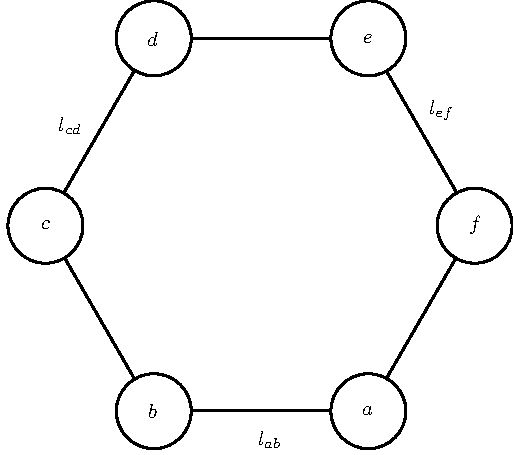
\includegraphics[width=4cm]{circle}
\label{subfiga}}
\hfill
\subfloat[Clique]{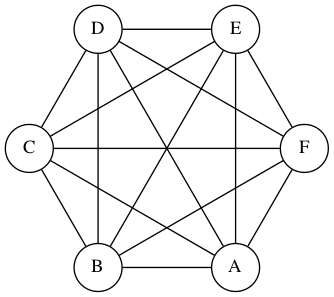
\includegraphics[width=4cm]{clique}
\label{subfigb}}
\caption{Circle and Clique topology of 6 nodes}
\vspace*{0.1in}
\end{figure}

For Case \Rmnum{1}.\Rmnum{1}, the adjusted link may be $l_{cd}$, the new bottleneck still be $l_{ab}$. 
The traffic on $l_{ab}$ is increased by the origin traffic on link $l_{cd}$, So we compute OPRE by:

\begin{equation}
\frac {\frac{dem_{ab} + dem_{cd}}{cap_{ab}}} {\frac{dem_{ab}}{cap_{ab}}} = 1 + \frac{dem_{cd}}{dem_{ab}}
\end{equation}

Because the old bottleneck is $l_{ab}$, so we have inequation:

\begin{equation}
\frac {dem_{cd}} {cap_{cd}} < \frac {dem_{ab}} {cap_{ab}}
\end{equation}

From Ineq. (14) we get:

\begin{equation}
\frac {dem_{cd}} {dem_{ab}} < \frac {cap_{cd}} {cap_{ab}}
\end{equation}

So we have OPRE in Case \Rmnum{1}.\Rmnum{1} combined by Eq. (13) and Ineq. (15):

\begin{equation}
1 + \frac {dem_{cd}} {dem_{ab}} < 1 + \frac {cap_{cd}} {cap_{ab}}
\end{equation}

For Case \Rmnum{1}.\Rmnum{2}, the adjusted link also be $l_{cd}$, but the new bottleneck may be $l_{ef}$.
Computing the OPRE similar as above:

\begin{equation}
\frac {\frac{dem_{ef} + dem_{cd}}{cap_{ef}}} {\frac{dem_{ab}}{cap_{ab}}} = 
\frac {dem_{ef} * cap_{ab}}{dem_{ab} * cap_{ef}} + \frac {dem_{cd} * cap_{ab}}{dem_{ab} * cap_{ef}}
\end{equation}

Because the old bottleneck is $l_{ab}$, so we have Ineq. (14) and :

\begin{equation}
\frac {dem_{ef}} {cap_{ef}} < \frac {dem_{ab}} {cap_{ab}}
\end{equation}

So we get inequation from Ineq. (18):

\begin{equation}
\frac {dem_{ef} * cap_{ab}} {dem_{ab} * cap_{ef}} < 1
\end{equation}

Also from Ineq. (14) we have :

\begin{equation}
\frac {dem_{cd} * cap_{ab}} {dem_{ab}} < cap_{cd}
\end{equation}

Combine Eq. (17), Ineq. (19) and Ineq. (20), we have OPRE in Case \Rmnum{1}.\Rmnum{2}:

\begin{equation}
\frac {dem_{ef} * cap_{ab}}{dem_{ab} * cap_{ef}} + \frac {dem_{cd} * cap_{ab}}{dem_{ab} * cap_{ef}} 
< 1 + \frac {cap_{cd}}{cap_{ef}}
\end{equation}

For Case \Rmnum{2}.\Rmnum{1}, the adjusted link may be $l_{ab}$, namely the old bottleneck link, the new bottleneck
maybe $l_{ef}$. Computing the OPRE similar as above:

\begin{equation}
\frac {\frac{dem_{ef} + dem_{ab}}{cap_{ef}}} {\frac{dem_{ab}}{cap_{ab}}} = 
\frac {dem_{ef} * cap_{ab}}{dem_{ab} * cap_{ef}} + \frac{cap_{ab}}{cap_{ef}} 
\end{equation}

Becuase the old bottleneck has the maximum link utilization, so combine Ineq. (19) and Eq.(22) we obtain OPRE in Case 
\Rmnum{2}.\Rmnum{1}:

\begin{equation}
\frac {dem_{ef} * cap_{ab}}{dem_{ab} * cap_{ef}} + \frac{cap_{ab}}{cap_{ef}} < 1 + \frac{cap_{ab}}{cap_{ef}}
\end{equation}


To sum up, we have inequation from Ineq. (16), Ineq. (21) and Ineq. (23):

\begin{equation}
1 + \max \{\frac{cap_{cd}}{cap_{ab}}, \frac{cap_{cd}}{cap_{ef}}, \frac{cap_{ab}}{cap_{ef}} \} < 1 + \frac{\max_{l \in E} cap_{l}}{\min_{l \in E} cap_{l}}
\end{equation}

\end{proof}

\section{}
\begin{proof}
The spanning tree of circle is the topology which lose one link. In Appendix. A, when we consider the robust routing, we adjust the traffic 
on one link to another path, it is similar that we switch off the link and forward the traffic to some other path. The complete proof is 
almost the same with Appendix. A.
\end{proof}

\section{}
\begin{proof}
Every link in the spanning tree will split the graph to two components, the flow between them must need trace this link.
we say the bottleneck link is $l_{ab}$ for optimal routing on the origin topology, and let $l_{ef}$ be the bottleneck link for 
the robust routing on the spanning tree. Other symbols are consistent with Appendix. A. So we have OPRE:

\begin{equation}
    \frac{\frac{\sum_{(i,j) \in E} dem_{ij}}{cap_{ef}}}{\frac{dem_{ab}}{cap_{ab}}} = \frac{cap_{ab}}{cap_{ef}} \sum_{(i,j) \in E} \frac{dem_{ij}}{dem_{ab}}
\end{equation}

Because the $l_{ab}$ is the bottleneck link, we have:

\begin{equation}
    \frac{dem_{ij}}{cap_{ij}} < \frac{dem_{ab}}{cap_{ab}}, \forall (i,j) \in E
\end{equation}

\begin{equation}
    \frac{dem_{ij} * cap_{ab}}{dem_{ab}} < cap_{ij}, \forall (i,j) \in E
\end{equation}

So we have OPRE:

\begin{equation}
    \frac{cap_{ab}}{cap_{ef}} \sum_{(i,j) \in E} \frac{dem_{ij}}{dem_{ab}} < \sum_{(i,j) \in E} \frac{cap_{ij}}{cap_{ef}}
\end{equation}

And we know that, the amount of $l_{ij}$ between two parts must less than $\frac{n^2}{2}$, so OPRE must lower than:

\begin{equation}
    \sum_{(i,j) \in E} \frac{cap_{ij}}{cap_{ef}} < \frac{n^2}{2} \frac{\max_{l \in E} cap_l}{\min_{l \in E} cap_l}
\end{equation}

\end{proof}

% that's all folks
\end{document}



























